%HEADER

%<---!!!!!!!!!!!!!!! MAKRO-DEFIONITIONEN; BITTE NICHT VERAENDERN !!!!!!!!!!
%<--- ARBEIT EINSEITIG
\def\makroEinseitig{
%KOMA-Script-Klasse: scrreprt
%deutsches Design, Schriftgröße 12, DIN A4
%Literaturverzeichnis und Index in Inhaltsverzerzeichnis einbinden
\documentclass[12pt,a4paper,listof=totoc,oneside]{scrreprt}
%Seitenspiegel einstellen
\usepackage[a4paper]{geometry}
\geometry{a4paper,left=30mm,right=25mm,
bottom=20mm,top=15mm,bindingoffset=2mm,
includehead,includefoot}}
% ARBEIT EINSEITIG --->

\def\makroZweiseitig{
%<--- ARBEIT ZWEISEITIG
%KOMA-Script-Klasse: scrreprt
%deutsches Design, zweiseitig
%Literaturverzeichnis und Index in Inhaltsverzerzeichnis einbinden
\documentclass[12pt,a4paper,listof=totoc,twoside, headsepline]{scrreprt}
\usepackage[a4paper]{geometry}
\geometry{a4paper,left=25mm,right=25mm,
bottom=20mm,top=15mm,bindingoffset=2mm,
includehead,includefoot}}
% ARBEIT ZWEISEITIG --->

%<--- Einstellungen Kopfzeile
\def\makroFH-Kopfzeilenstil{
\pagestyle{scrheadings} 
\setheadsepline{0.4pt}
\pagestyle{scrheadings}
\renewcommand*{\chapterpagestyle}{scrheadings}}
%Einstellungen Kopfzeile --->
%!!!!!!!!!!!!!!! MAKRO-DEFIONITIONEN; BITTE NICHT VERAENDERN !!!!!!!!!!--->


%AUSWAHL: TEXT EINSEITIG (ja/nein)
%\makroEinseitig
\makroZweiseitig

%schalte Umlaute frei
\usepackage[english, ngerman]{babel}
%passende Codierung
\usepackage[utf8]{inputenc}
%Seitenspiegel einzustellen
\usepackage[a4paper]{geometry}

%%%%%%%%%%%%%%%%%%%%%%%%%%%%%%%%%%%%%%%%%%%%%%%%%%%%%%%%%%%%%%%%%%%%%%%%%%%%%%%%
% Deutsche und englische Referenzen
\usepackage{babelbib}

% Utopia Schriftart (obsolet)
%\usepackage{utopia}
% jetzt... 
\usepackage{fourier}

% Farbige Überschriften
% https://www.overleaf.com/learn/latex/Using_colours_in_LaTeX
\usepackage[dvipsnames]{xcolor}
\usepackage{sectsty}
\chapterfont{\color{CornflowerBlue}}
\sectionfont{\color{Cerulean}}
\subsectionfont{\color{Cerulean}}
\subsubsectionfont{\color{Cerulean}}
\paragraphfont{\color{Cerulean}}
%%%%%%%%%%%%%%%%%%%%%%%%%%%%%%%%%%%%%%%%%%%%%%%%%%%%%%%%%%%%%%%%%%%%%%%%%%%%%%%%

%Mathepaket
\usepackage{amsmath}
%Symbole
\usepackage{amssymb}
%griechische Symbole
\usepackage{upgreek}
%weitere Symbole
\usepackage{pxfonts}
% Phonetischen Alphabete für LaTeX
\usepackage{tipa}
%farbige Schriften
%\usepackage{color}
\usepackage{scrhack}
%Bilder fixieren
\usepackage{float}
%Grafiken einbinden
\usepackage{graphicx}
% Kopf- und Fußzeilen
\usepackage[automark,standardstyle,markusedcase]{scrlayer-scrpage}
% deutsche Überschriften
\usepackage[ngerman]{translator}
% Kopfzeilenabstand festlegen
\setlength{\headheight}{10mm}
%Abb. statt Abbildung
\usepackage{caption3}
\addto\captionsngerman{
\renewcommand{\figurename}{Abb.}
\renewcommand{\tablename}{Tab.}
}
%Glossar-Pakage
% HYPERREF VOR GLOSSARIES EINFÜGEN
\usepackage{hyperref}

\usepackage[
nonumberlist, %keine Seitenzahlen anzeigen
acronym,      %ein Abkürzungsverzeichnis erstellen
toc]          %Einträge im Inhaltsverzeichnis      
{glossaries}
\usepackage{cite}
% degree sign
\usepackage{gensymb}

\hypersetup{ colorlinks,
linkcolor=MidnightBlue,
filecolor=MidnightBlue,
urlcolor=MidnightBlue,
citecolor=MidnightBlue }

%Glossar einschalten
\makeglossaries


%fertigen Kopfzeilenstil aktivieren
\makroFH-Kopfzeilenstil

%Zeilenabstand * 1.25 (default)
\renewcommand{\baselinestretch}{1.25}\normalsize
%(Kommentar entfernen, um Zeilenabstand
% auf 1,5-fache Groesse zu ueberschreiben)
%\renewcommand{\baselinestretch}{1.50}\normalsize

% KOMPILATION
% pdflatex Arbeit_Main.tex
% makeglossaries Arbeit_Main
% bibtex Arbeit_Main
% 2 * pdflatex Arbeit_Main.tex
%

% https://www.overleaf.com/learn/latex/Tables
%\setlength{\arrayrulewidth}{0.5mm}
\setlength{\tabcolsep}{18pt}
\renewcommand{\arraystretch}{1.5}

\newcommand{\todo}[1]{\textcolor{red}{\textbf{TODO #1}}}
\newcommand{\xcom}{\textcolor{YellowGreen}{\textbf{[?] }}}
\newcommand{\misobj}[1]{\textcolor{YellowGreen}{\textbf{#1}}}

\begin{document}

%Befehle für Symbole
%\newglossaryentry{symb:Pi}{
%name=$\pi$,
%description={Die Kreiszahl.},
%}
%\newglossaryentry{symb:Phi}{
%name=$\varphi$,
%description={Ein beliebiger Winkel.}
%}
%\newglossaryentry{symb:Lambda}{
%name=$\lambda$,
%description={Eine beliebige Zahl, mit der der nachfolgende Ausdruck
%multipliziert wird.}
%}

%Akronyme
\newacronym{MS}{MS}{Microsoft}
%\newacronym{CD}{CD}{Compact Disc}
%Eine Akronym mit Glossareintrag
%\newacronym{AD}{AD}{Active Directory\protect\glsadd{glos:AD}}

%Glossareinträge
%\newglossaryentry{glos:AD}{
%name=Active Directory,
%description={Active Directory ist in einem Windows 2000/" "Windows
%Server 2003-Netzwerk der Verzeichnisdienst, der die zentrale ...
%}
%}
\newglossaryentry{glos:AntwD}{name=Antwortdatei, description={Informationen zum
Installieren einer Anwendung oder des Betriebssystems.}}




%Titelseite
% Seitennummer aus
\thispagestyle{empty}
\begin{titlepage}
	\vspace{3cm}

%%\begin{center}
%%	\Huge	
%%	HOCHSCHULE LANDSHUT \\
%%	\Large
%%	FAKULTÄT INFORMATIK
%%\end{center}

%%\vspace{1cm}

\begin{center}
	\includegraphics[scale=0.8]{Grafiken/hl-logo.pdf}  
\end{center}

\vspace{2.5cm}

\begin{center}
  \Large FAKULTÄT INFORMATIK
\end{center}

\vspace{1cm}
\begin{center}
	\Huge
	\textbf{Masterarbeit}\\
\end{center}

\vspace{1cm}

\begin{center}
	\Large
	\textsc{Predictive Analytics im öffentlichen Sektor - Anwendungsmöglichkeiten,
    Chancen und Risiken}\\
\end{center}

\vspace{1.5cm}

\begin{center}
	\Large
	Dmitrij Novikov
\end{center}

\vspace{2cm}
\begin{center}
	\large
	%\the\month\,/\,\the\year
  \today
\end{center}

\vspace{2cm}
\begin{center}
	\large
	Betreuer: Prof. Dr. Wunderlich
\end{center}

\end{titlepage}


%Füge leere Seite ein (optional)
\input{Inhalt/LeereSeite}
%Verwende Muster-Erklärung zur selbstständigen Arbeit 
\input{Inhalt/Erklaerung}
%Füge leere Seite ein (optional)
\input{Inhalt/LeereSeite}

\begin{abstract}
\begin{center}
\Huge
\emph{\textbf{Übersicht}}
\end{center}
\normalsize
\vspace{15mm}
\textit{Forecasting und Predictive Analytics sind zwei evidenzbasierte Methoden,
die helfen können, bessere Urteile zu fällen und bessere Entscheidungen zu
treffen. Allerdings wird die Verbreitung dieser Methoden auf taktischer und
strategischer Ebene schwierig werden, da insbesondere dort Widerstände zu
erwarten sind. Es bleibt zu hoffen, dass der Wille, bessere 
Entscheidungsgrundlagen zu erhalten, stärker ist. Eine Literaturrecherche 
zu der Verbreitung von Predictive Analytics im öffentlichen Sektor ergab, dass
solche Anwendungen hauptsächlich auf operativer Ebene implementiert werden und
bestätigte damit obigen Verdacht.}
\end{abstract}


\setcounter{page}{1}
\tableofcontents


\chapter{Einleitung}
\label{part:Einleitung}

In dieser Arbeit soll die Anwendung von Datenanalysen und insbesondere
von \emph{\gls{glos:Predictive_Analytics}} im öffentlichen Sektor untersucht
werden.
Der Schwerpunkt liegt dabei auf Deutschland, wobei aber auch relevante
Anwendungsgebiete in anderen Staaten betrachtet werden. \\ \\
Der einleitende Teil~\ref{part:Schw_Vorhersagen} soll zunächst das Problem der
Schwierigkeit von
Prognosen untersuchen und damit eine Motivation für die Anwendung von 
\emph{predictive analytics} liefern. \\ \\
In Teil~\ref{part:Konzepte_PA} werden die wichtigsten Konzepte von
\emph{predictive analytics} vorgestellt. Dabei werden auch die allgemeinen
Risiken bei der Anwendung diskutiert. \\ \\
\misobj{weitere Teile}

\chapter{Die Schwierigkeit von Vorhersagen}
\label{part:Schw_Vorhersagen}

Mit Hilfe von \emph{\gls{glos:Predictive_Analytics}} werden Datenanalysen
erstellt, die die Vorhersage von Entwicklungen oder die Einschätzung von
Situationen unterstützen sollen. Dabei werden in der Regel Computeralgorithmen
mit Daten trainiert, um für spätere Abfragen zuverlässige Prognosen zu liefern.
Entscheidungsträgern soll \emph{predictive analytics} also helfen, bessere
strategische Entscheidungen zu treffen (vgl. \cite{Mauerer}, S.~2). %\\ \\
Dies könnte
\begin{description}
\item[(a)] notwendiger sein als erwartet und
\item[(b)] schwieriger werden als gedacht.
\end{description}
Denn eine ausführliche Studie des Psychologen Philip Tetlock aus dem Jahr 2005
(siehe \cite{Tetlock}) ergab,
dass Experten zu politischen Fragen keine besseren Prognosen liefern konnten,
als die einfachsten statistischen Algorithmen. Zudem hatten die Experten
große Schwierigkeiten damit, ihre Prognosen angesichts schlechter Resultate
anzupassen und zu verbessern. \\ \\
Die Experten sollten ihr Können bei mehreren Prognoseaufgaben
(\emph{forecasting exercises}) unter Beweis stellen. Dabei wurden verschiedene
mögliche politische oder wirtschaftliche Ereignisse skizziert und die Experten
sollten subjektiv abschätzen, für wie wahrscheinlich sie es halten, dass das
Ereignis eintritt\footnote{Es sollten numerische Werte angegeben werden. Also
0 für \glqq{Es} ist unmöglich, dass das Ereignis eintritt\grqq und 1 für
\glqq{Das} Ereignis wird mit Sicherheit eintreten\grqq. Werte zwischen 0 und 1
drücken dann einen Grad von Unsicherheit über das Ereignis aus.}.
Nachdem das festgelegte Zeitfenster für die Ereignisse abgelaufen war, konnte
das Eintreten oder Nichteintreten der jeweiligen Szenarien beobachtet werden und
rückblickend mit den Vorhersagen der Teilnehmer abgeglichen werden.  
Zur Messung der Genauigkeit der Vorhersagen wurde eine Maßzahl,
der \emph{probability score} verwendet. Dadurch konnten die Vorhersagen der
menschlichen Teilnehmer mit den Ergebnissen von einfachen und erweiterten
statistischen Algorithmen verglichen werden. \\ \\
Das Ergebnis ist in Abbildung~\ref{pic:Tetlock_1} dargestellt und wird im
folgenden Text ausführlich erläutert\footnote{Die Grafik ist eine leicht 
abgewandelte Version vom Original aus \cite{Tetlock}, S. 51).}. \\ \\
\begin{figure}%[!hbt]
\centering
\caption{Bei den \emph{forecasting exercises} erzielte Wertungen.}

\includegraphics[scale=1.0]{Grafiken/Tetlock_1_Fertig_Ink.pdf} 
\label{pic:Tetlock_1}
\end{figure}
Die zwei
Bestandteile des \emph{probability score}, Kalibrierung (\emph{calibration}) und
Diskriminierung (\emph{discrimination}), sind auf den Achsen abgebildet. \\ \\ 
Kalibrierung (horizontale Achse) misst die Fähigkeit eines Prognostikers,
Ereignisse korrekt nach ihrer
Auftrittswahrscheinlichkeit zu ordnen (vgl. \cite{Tetlock}, S.~47). So ist ein
Prognostiker gut kalibriert, wenn etwa 10~\% der Ereignisse eintreten, für die
er eine Wahrscheinlichkeit von 0.1 geschätzt hat, 20~\% der Ereignisse eintreten
die eine Wahrscheinlichkeit von 0.2 erhalten haben, und so weiter. Je kleiner
der numerische Wert der Kalibrierung, desto besser ist der Prognostiker. Bei
einem Wert von 0 ist die bestmögliche Kalibrierung erreicht und aus diesem Grund
ist (1 - Kalibrierung) auf der horizontalen Achse abgebildet. \\ \\
Weiterhin ist ein Prognostiker umso besser bei der Diskriminierungskomponente
(vertikale Achse),
je eher es ihm gelingt die Auftrittswahrscheinlichkeiten von einzelnen
Ereignissen von der relativen Häufigkeit aller Ereignisse\footnote{
genauer: Das Verhältnis der Anzahl der eingetretenen Ereignisse zu der
Gesamtanzahl der Ereignisse} (\emph{base-rate})
zu unterscheiden. Perfekte Diskriminierung wird erreicht, wenn allen 
eingetretenen Ereignissen eine Wahrscheinlichkeit von 1.0 zugeordnet wird, und
alle Ereignisse, die nicht eingetreten sind, mit Null bewertet werden
(vgl. \cite{Tetlock}, S.~47).\\ \\
Nun gehen Kalibrierung und Diskriminierung als Summe in den
\emph{probability score} ein. Aus diesem Grund kann sich für verschiedene
Werte von Kalibrierung und Diskriminierung der gleiche Wert für den
\emph{probability score} ergeben. Die diagonalen Linien in Abbildung~\xcom
markieren Stellen mit konstantem \emph{probability score}. Je weiter rechts oben
eine Linie verläuft, desto höher ist der zugehörige \emph{probability score}.
\\ \\
Die Gesamtergebnisse für Kalibrierung und Diskriminierung für die verschiedenen
Teilnehmergruppen sind in der Graphik eingetragen. Die am besten qualifizierte
Gruppe stellen die Experten dar, die Fragen zu ihren jeweiligen Fachgebieten
erhalten haben (vgl. \cite{Tetlock}, S.~242). Weniger qualifiziert sind die 
\glqq{Dilettanten}\grqq (\emph{dilettantes}), Experten, die jedoch Fragen
beantwortet haben, die nicht zu ihrem Spezialgebiet gehören. Die Dilettanten
gaben an, dass sie sich mit Hilfe qualititativ hochwertiger Quellen
(\emph{Economist}, \emph{Wall Street Journal}, \emph{New York Times} etc.) über
Themen außerhalb ihrer Fachgebiete informieren (vgl. \cite{Tetlock}, S.~56).
Die Gruppe mit der geringsten Qualifikation waren Studenten, die die Übungen
zu Vorhersagen absolvieren mussten, nachdem sie kurze Zusammenfassungen von
Fakten zu den jeweiligen Themen erhalten haben (vgl. \cite{Tetlock}, S.~56).
\\ \\
Weiterhin enthält Abbildung~\ref{pic:Tetlock_1} auch die Ergebnisse, die von den
statistischen Algorithmen erzielt wurden. Zur besseren Übersicht werden die
Algorithmen hier in vier Gruppen eingeteilt. Der Stufe 0 Algorithmus würfelt
einfach die Antworten , er ordnet den zur Debatte stehenden Ereignissen
zufällige Wahrscheinlichkeiten zu. Weiterhin gibt es mehrere Varianten von
Stufe 1 Algorithmen, die als Antwort auf die Fragen immer die relative
Häufigkeit der Ereignisse eintragen. Etwas komplexer sind die Stufe 2
Algorithmen. Diese extrapolieren aus der Vergangenheit in die Zukunft und setzen
die Wahrscheinlichkeiten für die Ereignisse entsprechend. Die höchste
Komplexität hat der Stufe 3 Algorithmus. Um die Eintrittswahrscheinlichkeiten
der Ereignisse zu ermitteln, nutzt dieser die Vergangenheitswerte mehrerer
Variablen, die eine hohe Vorhersagekraft besitzen.\footnote{Die genaue Zuordnung
der Stufen 0-3 zu den Algorithmen in der Originalquelle (\cite{Tetlock}, S.~51)
sieht folgendermaßen aus:
\begin{description}
\item[Stufe 0:] \emph{random guessing} (\emph{chimp})
\item[Stufe 1:] \emph{contemporary base rate} (1-1), \emph{restrictive base
  rate} (1-2), \emph{expansive base rate} (1-3)
\item[Stufe 2:] \emph{cautious case-specific extrapolation} (2-1),
  \emph{aggressive case-specific extrapolation} (2-2)
\item[Stufe 3:] \emph{autoregressive distributed lag models}
\end{description}
} \\ \\
Abbildung~\ref{pic:Tetlock_1} zeigt, dass die Experten die Studenten bei
den \emph{forecasting exercises} deutlich schlagen konnten. Allerdings waren die
Experten kaum besser (!) als der zufallsgesteuerte Algorithmus 
(Stufe 0)\footnote{Die Experten waren schlechter kalibriert aber besser bei
der Diskriminierung, sodass sie insgesamt eine etwas bessere Gesamtwertung
hatten}. Insbesondere verloren die Experten gegen die komplexeren Algorithmen
(Stufe 2 und 3) mit deutlichem Abstand und zwar sowohl bei Kalibrierung, als
auch bei Diskriminierung. Falsche Überzeugungen und mentale Barrieren haben, so
Tetlock, das Urteilsvermögen der Experten getrübt und zu den schlechten
Ergebnissen geführt (mehr dazu in Abschnitt~\xcom). \\ \\
Was haben diese Ergebnisse mit \emph{predictive analytics} und dem öffentlichen
Sektor zu tun?\\ \\
Erstens waren die Fragestellungen der \emph{forecasting exercises} aus den
Bereichen Politik und Wirtschaft\footnote{
Andere Themen, wie beispielweise naturwissenschaftliche Fragestellungen,
z. B. \glqq{Wie} wahrscheinlich ist die Detektion dunkler Materie
in den nächsten fünf Jahren?\grqq, wurden nicht behandelt.
}, was für den öffentlichen Sektor relevant ist. Zweitens handelt es sich dabei
um generelle Probleme der menschlichen Urteilsfindung. Probleme, die in vielen
Bereichen auftreten und zu Fehleinschätzungen führen können. Zudem
konnten datenbasierte Algorithmen, also \emph{predictive analytics}, die
menschlichen Vorhersagen bei den \emph{forecasting exercises} schlagen. Dies
deutet darauf hin, dass formale Methoden wie \emph{predictive analytics} dabei
helfen können, bessere Urteile zu fällen und folglich auch bessere
Entscheidungen zu treffen. \\ \\
Der nächste Teil der Arbeit behandelt \emph{predictive analytics},
den Prozess der (menschlichen) Urteilsfindung und wie formale Methoden diesen
Prozess verbessern können.


\chapter{Konzepte von Predictive Analytics}
\label{part:Konzepte_PA}

\section{Begriffsdefinition und -Abgrenzung}

\section{Bestandteile von Predictive Analytics}

\subsection{CRISP-DM Vorgehensmodell}

\subsection{Daten}

\subsubsection{Information Management (Data Warehouse)}

\subsubsection{Datenabhängige Ziele}

\paragraph{\ldots}

\paragraph{Beschreibung der Daten}

\paragraph{Klassifikation}

\paragraph{Zeitreihenanalyse}

\subsection{Methoden}

\subsubsection{Die Großen Drei}

\paragraph{Regression}

\paragraph{Entscheidungsbäume}

\paragraph{Neuronale Netze}

\subsubsection{Zeitreihenanalyse}

\subsubsection{\ldots}

\subsection{Werkzeuge}

\subsection{(Kreative) Freiheitsgrade bei der Implementierung eines
  Vorhersagemodells}

\section{Anwendungsbeispiele}

\subsection{Allgemeine Anwendungsfelder (siehe SAP Artikel)}

\subsection{\ldots}

\section{Allgemeine Risiken bei der Nutzung von Predictive Analytics}

Es exisitieren Risiken, die dazu führen können, dass die Ziele einer
Datenanalyse nicht oder nicht in vollem Umfang erreicht werden können.
Im folgenden Text werden einige dieser Risiken erläutert.

\subsection{Risiko der Unverhältnismäßigkeit}

Die Anwendung von Predictive Analytics ist mit einem hohen Aufwand verbunden.
Dabei spielen die Kosten für die Datenerhebung eine wesentliche Rolle.
Zusätzlich werden für die Datenanalyse Kenntnisse aus verschiedenen
Fachrichtungen benötigt. So sind einerseits anwendungsspezifische Kenntnisse
zur Interpretation der Daten und der Ergebnisse wünschenswert. Andererseits
werden zur Durchführung der Datenanalyse Kenntnisse in Mathematik, Statistik und
Informatik benötigt. \\ \\
Aus diesem Grund besteht das Risiko, dass die Kosten einer Anwendung von
Predictive Analytics den Nutzen übersteigen. Es ist auch möglich, dass das
gleiche Ergebnis mit einer einfacheren, kostengünstigeren Methode erreicht
werden kann. In diesem Fall würde die Anwendung eines aufwändigen Predictive
Analytics Verfahrens wertvolle Ressourcen binden, die an anderer Stelle stärker
gebraucht werden. \\ \\
Somit ist es wichtig, Betrachtungen zu Alternativkosten \todo{gls eintrag}
in die 
Planung von Predictive Analytics Anwendungen einzubeziehen. 

\subsection{Risiken bei der Datenerhebung}

\subsubsection{\ldots}

\subsection{Risiken bei der Interpretation der Daten}

\subsection{Risiken bei der Interpretation der Ergebnisse}

Wenn die Ergebnisse der Datenanalyse zur Entscheidungsunterstützung herangezogen
werden, beeinflussen sie das Verhalten der Entscheidungsträger. Dies kann zur
Entstehung problematischer psychosozialer Effekte führen. Zwei Beispiele hierfür
werden nun erläutert.

\subsubsection{Prognose verändert das Verhalten des Systems 
%  (``Selffulfilling Prophecy'')}
  (\glqq{Selffulfilling} Prophecy\grqq)}

\subsubsection{Ignorieren der Unsicherheiten bei der Prognose}

Es besteht die Gefahr, dass die Unsicherheiten von Vorhersagen ignoriert werden
und die Prognose als eine Gewissheit betrachtet wird. Somit wird möglichen,
alternativen Entwicklungen bei der Entscheidungsfindung nicht genügend Bedeutung
beigemessen. Dies kann dazu führen, dass Risiken falsch kalkuliert werden und
in der Zukunft nicht genügend Handlungsoptionen zur Verfügung stehen.


\chapter{Predictive Analytics im öffentlichen Sektor}

Bei der folgenden Analyse ist es sinnvoll zwischen strategischer, taktischer und
operativer Ebene zu unterscheiden. Im Allgemeinen lassen sich die verschiedenen
Ebenen wie folgt abgrenzen:

\begin{description}

\item[Strategische Ebene:] \hfill \\
Bei der strategischen Ausrichtung einer Organisation werden allgemeine, wegweisende Ziele definiert
und es werden den Zielen Prioritäten zugewiesen. Strategische Entscheidungen werden in 
der Regel vom Top Management gefällt. Im öffentlichen Sektor sind führende Politiker, 
wie beispielsweise Minister, und hohe Staatsbeamte die Entscheidungsträger auf dieser Ebene.
Die politische Weltanschauung der Entscheidungsträger hat auf dieser Ebene den 
meisten Einfluss auf die gewählten Ziele und ihre Prioritäten.

\item[Taktische Ebene:] \hfill \\
Die Aufgabe der taktischen Ebene ist die Entwicklung eines Vorgehens, das es
ermöglicht, die strategischen Ziele der Organisation zu erreichen. Die strategischen
Prioritäten sollten dabei, wenn möglich, ebenfalls eingehalten werden. Entscheidungen
auf der taktischen Ebene werden vom mittleren Management und seltener auch vom Top
Management getroffen. Staatsbeamte im mittleren und gehobenen Dienst, sowie Projektmanager von
Unternehmen, die öffentliche Aufträge bearbeiten, sind die Entscheidungsträger auf der taktischen
Ebene im öffentlichen Sektor. Die politische Weltanschauung der Entscheidungsträger hat 
auf die taktische Ebene weniger Einfluss als auf die strategische Ebene. 

\item[Operative Ebene:] \hfill \\
Entscheidungsträger auf der operativen Ebene haben die Aufgabe das \glqq{Tagesgeschäft}\grqq{}
zu überwachen und sicherzustellen, dass die Vorgaben der taktischen Ebene eingehalten werden.
Das operative Management und auch Angestellte ohne besondere Führungsaufgaben treffen operative
Entscheidungen, wobei ihr Spielraum dabei durch die Entscheidungen der strategischen und taktischen
Ebene meist stark eingeschränkt ist. Im öffentlichen Sektor führen Beamte im mittleren Dienst und 
operative Manager von Firmen mit öffentlichen Auftraggebern Tätigkeiten auf operativer Ebene aus.


\end{description}

% TODO
% Stand Entscheidungshilfen (wie vorstellbar: Mensch entscheidet, Computer
%   unterstützt)
% Abgrenzung zum privaten Sektor
% auf operativer Ebene allerdings ähnlich
% unterschied strategisch, taktische Ebene, operativ
% top management, mittleres management, operatives management 
% s. Watson, Abschnitt Lack of regulation and algorithm bias
% TODO bias insgesamt (in Rahmenbedingungen)
\begin{figure}%[!hbt]
\centering
\caption{Risikomatrix für die Nutzung maschineller Entscheidungshilfen}
\includegraphics[scale=1.0]{Grafiken/Risk_Matrix_Ink.pdf} 
\label{pic:Risiko_Matrix}
\end{figure}

\section{Rahmenbedingungen}

% TODO Technologie prinzipiell kein Hindernis (s. IT Novum)

% TODO
% Politiker, Experten und Kommentatoren formulieren keine subjektiven Wsk und
% niemand berechnet den Brier Score (oder ein anderes Maß)
% Widerstände auf strat und takt Ebene gegen Forecasting und PA
% Forecasting und PA nicht auf dem Vormarsch
% Forecasting leichter zu sehen,
% PA auf operativer Ebene (Tabellenkalkulation) verschleiert Widerstand auf
% takt und strategischer Ebene (!)
% Rahmenbedingungen:
% - Wahrheit taktisch genutzt
% - versch. Gruppen/Kulturen -> versch. Wahrheiten
% - Themen kontroverser (vs. z. B. Fruchtsäfte)
% - Konkurrenz (v. a. bei strategischen Entscheidungen) 
% - Ignorieren (-> Probleme menschl. Urteile)

%-------------------------------------------------------------------------------
Tetlock ist der Meinung, dass die Kernaufgabe politischer Weltanschauungen
nicht die Erstellung möglichst korrekter Prognosen ist, sondern die
Aufrechterhaltung einer bequemen Illusion von Berechenbarkeit
(vgl. \cite{Tetlock}, S.~39). Somit sind die Ergebnisse schlecht, weil keine
genaue Abbildung der Realität beabsichtigt wird. Die Aufrechterhaltung von
Glaubenssätzen, die zum kollektiven Zusammenhalt beitragen, hat höhere
Priorität.

In diesem Zusammenhang sind auch verschiedene Interpretationen des
Wahrheitsbegriffs bedeutsam. Eine weit verbreitete Interpretation wird mit
Hilfe des Pragmatismus von William James definiert. Demnach werden
Aussagen von Menschen als Wahrheit akzeptiert, falls die Aussagen ihnen bei der
Orientierung in der Welt nützlich sind. Dies liefert eine Erklärung dafür, dass
Menschen dazu tendieren Aussagen zu glauben, die ihre eigene Weltsicht
bestätigen. Bei einer extremen Ausprägung des pragmatischen Wahrheitsbegriffs
wird aus der Nützlichkeit einer Aussage ihr Wahrheitsgehalt abgeleitet:
\glqq{Es ist wahr, weil es nützlich ist}\grqq. (vgl. \cite{Precht})

Diese radikale Wahrheitsinterpretation ist problematisch, wenn die als Wahrheit
betrachteten Grundsätze der Realität widersprechen. Denn es gibt keine
Möglichkeit, die Grundsätze mit Hilfe von empirischen oder logischen Beweisen
zu revidieren und an die Realität anzupassen. Langfristig führen falsche
Grundsätze somit zu schlechtem Urteilsvermögen, was wiederum zu schlechten
Entscheidungen führt. Insbesondere sind Datenanalysen in einer solchen Situation
nicht zweckdienlich, da Ergebnisse selektiv ignoriert oder abgelehnt werden.

Eine andere Interpretation von Wahrheit legt großen Wert auf die Beweisbarkeit
von Aussagen. Eine solche Interpretation ist beispielsweise in der Wissenschaft
verbreitet. Aussagen wird erst dann ein Wahrheitswert zugewiesen, wenn
unwiderlegbare Beweise für die Gültigkeit der Aussage vorhanden sind. Eine
solche Interpretation weicht stark vom pragmatischen Standpunkt ab, kann aber
ebenfalls problematisch werden. Es besteht die Gefahr sich bei der Prüfung von
Aussagen in Kleinigkeiten zu verlieren, handlungsunfähig zu werden oder
nützliche Erkenntnisse zu lange anzuzweifeln\footnote{
Beispiele für Zweifel, die gefährlich werden, weil sie Fortschritt blockieren
sind auf Seite~\xcom erläutert.
}.

Vermutlich ist für ein gutes Urteilsvermögen ein nüchterner Pragmatismus
notwendig, bei dem vorsichtig zwischen Nutzen und Wahrheit abgewogen wird und
auch unangenehme Meinungen als Wahrheit akzeptiert werden können.
Bedauerlicherweise gerät ein solcher Pragmatismus mit jeder, insbesondere
politischen, Weltanschauung in Konflikt, die selbst nicht in ähnlicher Weise
pragmatisch ist.

%-------------------------------------------------------------------------------

\subsection{Eine pessimistische Sichtweise}

Je mehr das Treffen von Entscheidungen zur Hauptaufgabe von Personen gehört,
desto stärker betrachten sie \emph{predictive analytics} als eine Gefahr für
ihren Arbeitsplatz.

Es gibt Stimmen, die behaupten, dass ein immenser Widerstand gegen die
Einführung solcher Methoden [Forecasting + Predictive Analytics] zu erwarten
ist. Teilweise deutet sich sogar eine Unmöglichkeit dieser Aufgabe an. Beim 
Thema Forecasting ist es Tetlock selbst, der sich skeptisch äußert. Er
benennt den Widerstand der Experten als die größte Barriere zur Einführung der
neuen Methodik (\emph{the most daunting of all the barriers to implementation},
vgl. \cite{Tetlock}, S.~235). Jackson und Reichin vertreten eine ähnliche
Auffassung (vgl. \cite{Jackson}, S.~295).

Der investigative Charakter von Datenanalysen kann Nervosität und Unbehagen
auslösen.

% TODO Daten (-> Heise) 
% Thapa_Parycek S. 46
\subsection{Eine optimistische Sichtweise}

% Formalisierung erwünscht (BBC + IC)

Bessere Prognosen und Urteile führen zu besseren Entscheidungen. Dies bringt
wiederum sowohl Vorteile gegenüber Konkurrenten als auch Vorteile bei der
Auseinandersetzung mit der \glqq{Natur}\grqq\footnote{
Genauer: Bei der Auseinandersetzung mit den Zwängen, die durch die Naturgesetze
und ökonomische Prinzipien definiert werden. Verzichtet man zum Beispiel auf das 
Rauchen kann es als eine gute Entscheidung betrachtet werden, da man dadurch
gesünder lebt. Hierfür muss zunächst erkannt werden, dass Rauchen ungesund ist.
Klingt heute einfach. Diese Erkenntnis zu erlangen war jedoch mit erheblichem
Aufwand verbunden, wobei auch wissenschaftliche und statistische Methoden
eine große Rolle spielten (vgl. zum Beispiel \cite{Proctor}).

Ein weiteres Beispiel für eine Entscheidung, die nicht in erster Linie Vorteile
gegenüber Konkurrenten verspricht, ist eine Entscheidung für eine bessere
Behandlungsmethode in der Medizin. Denn der primäre Zweck davon ist, 
mehr Menschen eine Heilung zu ermöglichen.
}

\section{Spieltheoretische Betrachtung}

Aufgrund der potentiell konfliktreichen Situation rund um die Einführung von
\emph{forecasting} oder \emph{predictive analytics}, bietet es sich an, die
\gls{glos:Spieltheorie} anzuwenden.

\subsection{Einleitung zur Spieltheorie}
% TODO


% deadlock (S. 218(
\begin{figure}%[!hbt]
\centering
\caption{Deadlock Auszahlungsmatrix}
\includegraphics[scale=0.8]{Grafiken/Deadlock_Ink.pdf} 
\label{pic:Deadlock}
\end{figure}

% stag hunt (S. 220)
\begin{figure}%[!hbt]
\centering
\caption{Stag Hunt Auszahlungsmatrix}
\includegraphics[scale=0.8]{Grafiken/Stag_Hunt_Ink.pdf} 
\label{pic:StagHunt}
\end{figure}

% mixed
\begin{figure}%[!hbt]
\centering
\caption{Gemischte 'Stag Hunt - Deadlock' Auszahlungsmatrix}
\includegraphics[scale=0.7]{Grafiken/Mixed_Ink.pdf} 
\label{pic:Mixed}
\end{figure}

\subsection{Kritische Würdigung der spieltheoretischen Betrachtung}

% TODO spielen implizit spieltheorie (s. Poundstone ?)

% prisoners dilemma (S.237)
% mixed
\begin{figure}%[!hbt]
\centering
\caption{Gefangenendilemma Auszahlungsmatrix}
\includegraphics[scale=0.8]{Grafiken/Prisoner_Ink.pdf} 
\label{pic:Prisoner}
\end{figure}

%-------------------------------------------------------------------------------
\section{Anwendungen von Predictive Analytics im öffentlichen Sektor}

% Auswahl
% TODO Fallstudien einfach ausführlichere Beispiele

\subsection{Daten}

% TODO
% 2 grundlegende Probleme
% - Datenschutz: Achtung Privatsphäre + Angst vor Missbrauch
% - Verzerrungen in Daten: insb. auch Big Data, Daten nicht repräsentativ,
%     Daten kulturabhängig

\subsection{Öffentliche Verwaltung}

% TODO
% Daten in der öffentlichen Verwaltung
% Open Data Portale ( GovData.de )
% Abgrenzung zu 'Nowcasting'
% Predictive Analytics in Finanzbehörden
% Predictive Policing
% Einschätzung der politischen Stimmungslage
% Vorhersage kultureller Unterschiede

\subsubsection{Predictive Analytics in der Steuerverwaltung}

Hier \cite{OECD}.

% TODO

% FTA: Forum on Tax Administration Survey (DE leider nicht dabei)

% EINSATZGEBIETE VON PA

% 1) Audit Case Selection

% hauptsächliches Anwendungsgebiet (S. 20)
%  prioritise cases for investigation, audits

%  social network analysis (für bestimmte fälle, z. B. VAT carousel fraud)(S. 21-22)
% identify risk groups where individual-level assessments may fail
% identify links between individuals, assemble connected individuals to visualised networks
% Analyse der networks (risk score) per Hand, rule based oder statistical model

% 2) Filing (Aktenablage) and payment compliance (S. 24)

% aim: secure outstanding payment or return or prevent the problem from occurring
% predictive: identify taxpayers who are likeliy to fail to meet their obligations
% prescriptive: how communicate most effectively with this group

% 3) Debt management (S. 26)

% resource priorization
% traditional: identify groups of potentially high-risk debtors
% new (u. A. uplift modelling): identify cases that are most likely to respond to
%   debt-management intervention

% 4) Taxpayer Service (S. 27)

% z. B. Text mining and sentiment analysis

% Text minining of inbound email in Singapore (S. 27-28)

% identify the nature of taxpayer inquiries
% example: identify common queries of taxpayers after policy has changed
%   -> able to react: infos on website, updates to taxpayers (vorsorglich)
% Text Mining replaced manual tracking of email enquiries + track enquiries more objectively

% 5) Policy evaluation (S. 28)

% most analytics work carried out to support operational decision-making
% but too for decision-making in relation to strategy and policy

% tax gap analysis (Steuerlücke), forecasting the impact of changes in tax policy

% (S. 29) 2012 model for assessment the effects of tax-reform on economy and social-welfare
% estimate economic and social consequences of tax reform, 
% report of analytics team played a key role in the policy reform process

% DATENPROBLEME

 % S. 51
% concerns about representativeness of data

% data from highly biased samples (alte interventionsfälle) -> nur kleiner ausschnitt aus gesamtpopulation

% selection effects -> biases

 % S. 52

% data from randomly selected audits in US to improve representativeness

% DATA COMPREHENSIVENESS (S. 52)

% data for analytics project from data collected and stored for
%   operational purposes

% -> missed opportunities: not useful information for operational purposes
%     (e. g. type of non-compliance in audit) but would be useful for analytical purposes
%     distinct models for each risk type possible

\subsubsection{Predictive Policing}

Grafik aus \cite{Bode}, S.~2.

\begin{figure}%[!hbt]
\centering
\caption{Predictive Policing Prozess}

\includegraphics[scale=1.1]{Grafiken/Predictive_Policing_Ink.pdf} 
\label{pic:Predictive_Policing}
\end{figure}

\subsubsection{Weitere Anwendungen}

\subsubsection{Cambridge Analytica - Fallstudie}

\begin{figure}%[!hbt]
\centering
\caption{Nutzung von Facebook Likes zur Vorhersage von Nutzerattributen}
\includegraphics[scale=1.0]{Grafiken/Facebook_Likes_Ink.pdf} 
\label{pic:Like_Matrix}
\end{figure}

\subsection{Gesundheit}

Diese Haltung war überraschend genug, um eine Nachfrage des Journalisten
auszulösen.

% TODO
% Google Flu Trends (vorerst gescheitert)
% Kohortenstudien nützlich bei: bsp. Kampagnen zur öffentlichen Gesundheit
%   bsp. Ernährungskampagnen, Anti-Rauch-Kampagnen 
% Kohortenstudien: nicht persönlich (s. Watson, Abschnitt Cohort treatment),
%   aber Sicherheitsbedenken bleiben (Anonymisierung nicht möglich, Sicherheits
%   risiken ...)
\subsubsection{Flint Trinkwasserskandal - Fallstudie}

\subsection{Bildung}

% Anwendungsbeispiel Decision Tree

% TODO echten Titel ersinnen
\chapter{Zusammenfassung und Fazit}

% TODO Interessantes
% inwiefern lassen sich kognitive Verzerrungen vermeiden (s. Anhang für
%   ein Paar Betrachtungen hierzu)

%%%%%%%%%%%%%%%%%%%%%%%%%%%%%%%%%%%%%%%%%%%%%%%%%%%%%%%%%%%%%%%%%%%%%%%%%%%%%%%%
\appendix

% TODO evtl umbennen 
\chapter{Forecasting - Technische Details}

Für Überprüfbarkeit:

Vollständig: Es gibt keine weitere Kategorie, in die ein Objekt (oder in diesem
Fall ein Ereignis) fallen könnte.

Gegenseitig ausschließend: ...

Die menschliche Intuition ist schlecht in Wahrscheinlichkeitsrechnung.

% TODO
% Brier Score Erklärung
% Brier Score Probleme
%   Vorhersage unwahrscheinlicher Ereignisse nicht gewürdigt
%   50/50 fence sitters -> unbefriedigend, Frustration (need for closure, S. 81)
%   % S. 276 Indiscriminate fence-sitting
% Bayes Belief Updating Erklärung/Herleitung
% Kognitive Verzerrungen, Auflistung, Diskussion
%   Erlernbar oder nicht (- individuell nicht gelungen, + in Gruppe, 
%     Kommunikation hilft, Unterschiede nicht unüberwindbar)
% + eher statistisch, mathematische "Verzerrungen" (subadditivity ...)
% 11 Commandments GJP

\section{Ten Commandments of Superforecasting}

Diese zehn Prinzipien für Forecasting können bei korrekter Anwendung die Genauigkeit von
Prognosen verbessern (vgl. \cite{Ten_Comm}). Eine kommentierte Version wird von Jackson und Reichin
angeboten (vgl. \cite{Jackson}, S.~292-294). Im folgenden Text werden diese zehn (eigentlich elf)
Prinzipien diskutiert:

\begin{description}

\item[(1) Triage:] \hfill \\
Diese Regel betrifft die Auswahl der Fragen, die man mit den Prognosen beantworten will und
der Ereignisse, die man vorhersagen will. So ist es nicht sinnvoll, sich mit sehr einfachen Fragen
oder Routinefragen zu beschäftigen, die mit Hilfe simpler Entscheidungsregeln beantwortet werden können.
Weiterhin macht es keinen Sinn, sich mit Fragen zu beschäftigen, die keine Relevanz haben. Schließlich
sollte man auch ein Gefühl dafür entwickeln, welche Prognosen notorisch fehleranfällig sind und damit
gemieden werden sollten.

Es ist auch wichtig auf die konkreten Fragestellungen bei den Prognosen zu achten, weil sich hier
eine Möglichkeit bietet, Vorhersagen zu verzerren. Die Art der Fragen und ihr \glqq{Schwierigkeitsgrad}\grqq{}
lassen sich nicht einschätzen, wenn lediglich der erreichte Brier Score zur Verfügung steht.
Unehrliche Forecaster können die erste Regel bewusst ausnutzen, indem sie die Auswahl der Fragen geschickt
manipulieren. Insbesondere können sie sich dadurch einen Vorteil gegenüber anderen Forecastern erschleichen,
die nicht den selben Satz an Fragen beantwortet haben. Es besteht grundsätzlich immer die Möglichkeit, dass
jemand den gleichen oder einen besseren Brier Score erreicht, weil er leichtere Fragen beantwortet hat.

\item[(2) Zerlegen von komplizierten Problemen in kleinere Teilprobleme:] \hfill \\
Diese Methode geht auf den Physiker Enrico Fermi zurück. Eine schwierige Frage, wie beispielsweise die
Frage nach der Anzahl der Klavierstimmer, die in Chicago leben, wird in kleinere Teilprobleme zerlegt:

\begin{description}

\item[(a)] Wie viele Klaviere gibt es in Chicago?
\item[(b)] Wie oft werden Klaviere jedes Jahr gestimmt?
\item[(c)] Wie lange dauert es ein Klavier zu stimmen?
\item[(d)] Wie viele Stunden im Jahr arbeitet ein Klavierstimmer durchschnittlich? 

\end{description}

Durch die Zerlegung in Teilprobleme werden getroffene Annahmen explizit gemacht, insbesondere können
fehlerhafte Annahmen besser erkannt werden. Schätzungen für die einzelnen Größen und damit für das Gesamtproblem
können erstellt und verschiedene Schätzungen miteinander verglichen werden. Dadurch kann der Grad der Unsicherheit
der Gesamtschätzung deutlicher herausgearbeitet werden.

\item[(3) Berücksichtigung von Basisraten:] \hfill \\
Dabei wird zwischen der Sicht von Außerhalb (\emph{outside view}) und der Sicht von Innerhalb (\emph{inside view})
unterschieden. Bei der Sicht von Außerhalb geht es darum, eine Basisrate für das spezifische Ereignis aufzustellen.
Die Kernfrage, die dabei beantwortet werden muss, lautet:

\begin{description}
\item[>] Wie oft geschehen Dinge dieser Art in ähnlichen Situationen?
\end{description}

Bei der Sicht von Innerhalb werden Eigenschaften gesammelt, die den konkreten Fall von vergleichbaren Fällen
unterscheiden. Diese neuen Variablen werden dann genutzt, um die Basisrate abzuändern und an die konkrete
Frage anzupassen.

Technischer ausgedrückt handelt es sich bei diesem Vorgehen um das Aufstellen eines Algorithmus, der auf Basisraten
basiert (siehe auch S.~\xcom). Zunächst wird anhand historischer Betrachtungen eine Basisrate aufgestellt, die
beschreiben soll, wie häufig Ereignisse dieser Art im Allgemeinen auftreten. Daraufhin werden Prädiktorvariablen gesucht, die
dafür verantwortlich sein können, dass die Häufigkeit eines Ereignisses von der allgemeinen Basisrate abweicht. Diese
Prädiktorvariablen werden dann gewichtet und mit der Basisrate verrechnet, wobei manche Prädiktoren das Ereignis wahrscheinlicher
machen, wohingegen andere die Warscheinlichkeit des betrachteten Ereignisses geringer machen.

\item[(4) Belief Updating:]
Gute Forecaster passen ihre Weltsicht ständig an neue Erkenntnisse an. Dabei geht es nicht nur darum die Formel von Bayes
(siehe S.~\xcom) anzuwenden. Vielmehr müssen zunächst wichtige Signale aus dem Fluss von Nachrichten herausgefiltert werden, wobei
Wunschdenken, Über- und Unterreaktionen vermieden werden müssen. Hierfür müssen Forecaster ständig die aktuellen Nachrichten beobachten 
und kritisch widerspiegeln.

\item[(5) Berücksichtigung rivalisierender Weltsichten:]
Hierbei geht es darum, den Wahrheitsgehalt zweier gegensätzlicher Meinungen in Verhältnis zueinander zu bringen (siehe S.~\xcom).


\end{description}

Wie in der Beschreibung angedeutet, versuchen manche Prinzipien die in Anhang~\xcom besprochenen Formeln in Worten zu beschreiben.

\chapter{Predictive Analytics mit R}

Hier ist die Intro \cite{Intro_R}.

% TODO

% organisations mature in R -> recruits from academia (R heavily used)
%    (OECD, S. 50) 

% TODO
% Kurzvorstellung R, Vergleich mit anderen Werkzeugen (insb. Python)
% vllt R stark in Grafik
% R Verwendung in Verwaltungen
% Grafik Skripte

%%%%%%%%%%%%%%%%%%%%%%%%%%%%%%%%%%%%%%%%%%%%%%%%%%%%%%%%%%%%%%%%%%%%%%%%%%%%%%%%
% TODO Bilder
% PA Schaubild
% Dataframe beispiel
% Predictive Policing Schaubild

% TODO vllt Zusatzmaterial:

% Tetlock S. 63: systematic distortions in the media markets for intellectual
%   commentary

% Bayes belief updating konvergiert (Arens)



%%%%%%%%%%%%%%%%%%%%%%%%%%%%%%%%%%%%%%%%%%%%%%%%%%%%%%%%%%%%%%%%%%%%%%%%%%%%%%%%
\listoffigures
\listoftables
\printglossary[title=Glossar]
\printglossary[type=\acronymtype, title=Akronyme]
% keine deutschen Überschriften
%\printglossaries 

\bibliography{Bibliographie/Bibli.bib}{}
\bibliographystyle{babplain}

\end{document}


